\documentclass[a4paper,12pt]{scrreprt}
\usepackage[T1]{fontenc}
\usepackage[utf8]{inputenc}
\usepackage[english]{babel}
\usepackage[table]{xcolor}% http://ctan.org/pkg/xcolor
\usepackage{tabu}
\usepackage{graphicx}
\usepackage{lmodern}
\usepackage{longtable}
\usepackage{morefloats}
\usepackage{comment}

\begin{document}

 
%\titlehead{Kopf} %Optionale Kopfzeile
\author{Ahmed Aly \and Helmut Brunner \and Stefan Pitirut } %3 Autoren
\title{TASK 02 Rock the net } %Titel/Thema
\subject{SEW} %Fach
%\subtitle{ } %Genaueres Thema, Optional
\date{\today} %Datum
\publishers{5AHITT} %Klasse

\maketitle
\tableofcontents


\chapter{Task}

\subsection{Basic tasks}

Implement a simple-to-use application to monitor and configure a hardware firewall appliance “Juniper NetScreen 5GT “. The firewall allows read access over the SNMP-protocol (your app should be able to test if SNMPv3 is available and if not fallback on SNMPv2c) and write access over Telnet.

Your app should accomplish following tasks:
\begin{itemize}

    \item List all configured firewall rules (policies) on the device, add the details of the mentioned services and zones as well.

    \item Allow refreshing of the list by clicking a button and by a configurable time-intervall. Your GUI should remain responsive even with short refresh-intervals!

    \item Visualize the thru-put for a highlighted firewall-rule (nice2have: multiple rows) in a line-chart (configurable refresh-interval, unit bytes/sec)

    \item Encapsulate the data retrieval for further reuse and easy expansion. An UML-model of your design will help you defend it at the review!

    \item Build a visual appealing and easy to use interface (there is more than Swing out there).
\end{itemize}
\subsection{Advanced tasks (obligatory for grades better than C)}

Additionally to the basic tasks your app should accomplish the following:
\begin{itemize}


    \item Alarm the user visually and per email if the config of the firewall-rules changes. To avoid polling use the SNMP-trap mechanism.

    \item Allow managing of firewall-rules (CRUD). To accomplish this, you will have to send configuration commands via telnet or ssh. An admin-account is available per request.

    \item Use multicast-groups to build a simple transaction system to serialize administrative tasks on the firewall (for example pass an “admin token” to recognize the collaborator who is allowed to write to the firewall). This should also work in a heterogenous environment (different implementations, different OSes), so you have to coordinate with other teams.

    \item Make sure, that your interface to the firewall allows an easy change of the firewall-model (new releases, manufacturer, ...). It is not necessary to make this configurable in the GUI but must (explicitly) be considered in your software-design!
\end{itemize}

	
\chapter{Design concept}
	SNMP Package:
	The SNMP package has an OIDEncoder, which defines the Standard OID's in static final variables. It is able to implement other IODEncoder, which have OID's for specific Routers. 
	The next step is to know what the returned values mean, this will be brovided by the class OIDInterpreter.
	\\
	The Factory pattern is used here to allow the class SNMPManager to use the right SNMP version. This pattern also allows the developer to add to SNMP version, if there are any new ones coming.
	\\
	The SNMP Manager sends a package with a specific OID and returns the receive message. This Class will be used as a Connector and a Receiver, which will be called by a command class.
	\\\\
	Command pattern:
	A command pattern is used to create specific actions, which can any connectors like SNMP, SSH or Telnet.
	\\\\
	Naturally there will be self written exceptions, which will be in the exceptions package.
	\\\\
	The Unit and GUI tests will be in a own test package.   
\chapter{User Stories}
As a user, I want to visually see the thru-put in bytes/sec as a chart on my Graphical User Interface.\\

As a user, I want to set the refresh-timer for the visualized thru-put on my Graphical User Interface.\\

As a user, I want to manually refresh the visualization for the thru-put on the Graphical User Interface.\\

As a user, I want to see the rules/zones/services of the firewall listed on the Graphical User Interface.\\

As a user, I want set the refresh-timer for the listing of the rules/zones/services of the firewall on the Graphical User Interface.\\

As a user, I want to manually refresh the listing of the rules/zones/services of the firewall on the Graphical User Interface.\\

As a user, I want to configure the application threw the Graphical User Interface.\\
\chapter{Libraries}
\begin{description}
\item The required libraries will be:
\begin{itemize}
\item SNMP4J
\item LOG4J
\item JUNIT
\item Mockito
\item Java Secure Channel (JSCH) |SSH|
\item JFreeSVG (charts)
\item JavaFX
\end{itemize}
\end{description}


\chapter{Diagrams}

\subsection{Policy Design}
The policy date will be shown in a table, which consists of 9 Elements. 
\begin{description}
\item The table header would look like this:\\
{policyId} | {policyName} | {policyServiceName} | {policySrcZone} | {policyDestZone} | {policySrcAddr} | {policyDestAddr} | {policyAction} | {policyStatus}
\item OIDs:\\
\begin{tabular}{l l l} 
policyId & .1.3.6.1.4.1.3224.10.1.1.1 & branch\\
policyName & .1.3.6.1.4.1.3224.10.1.1.24 & branch\\
policyServiceName & .1.3.6.1.4.1.3224.10.1.1.25 & branch\\
policySrcZone & .1.3.6.1.4.1.3224.10.1.1.3 & branch\\
policyDestZon & .1.3.6.1.4.1.3224.10.1.1.4 & branch\\
policySrcAddr & .1.3.6.1.4.1.3224.10.1.1.5 & branch\\
policyDestAddr & .1.3.6.1.4.1.3224.10.1.1.6 & branch\\
policyAction & .1.3.6.1.4.1.3224.10.1.1.8 & branch\\
policyStatus & .1.3.6.1.4.1.3224.10.1.1.23 & branch\\
\end{tabular}

\end{description}
The next step is to draw a chart with the thru-put of the firewall-rule in a line-chart, which is possible with the value policyBps. 

\begin{description}
\item OID:\\
\begin{tabular}{l l l} 
policyBps & .1.3.6.1.4.1.3224.10.2.1.6 & branch\\
\end{tabular}
\end{description}

\subsection{UML Class Diagram}

\begin{figure}[h!]
\centering
\caption{UMLClass Diagram}
\label{fig:RTNUmlImage}
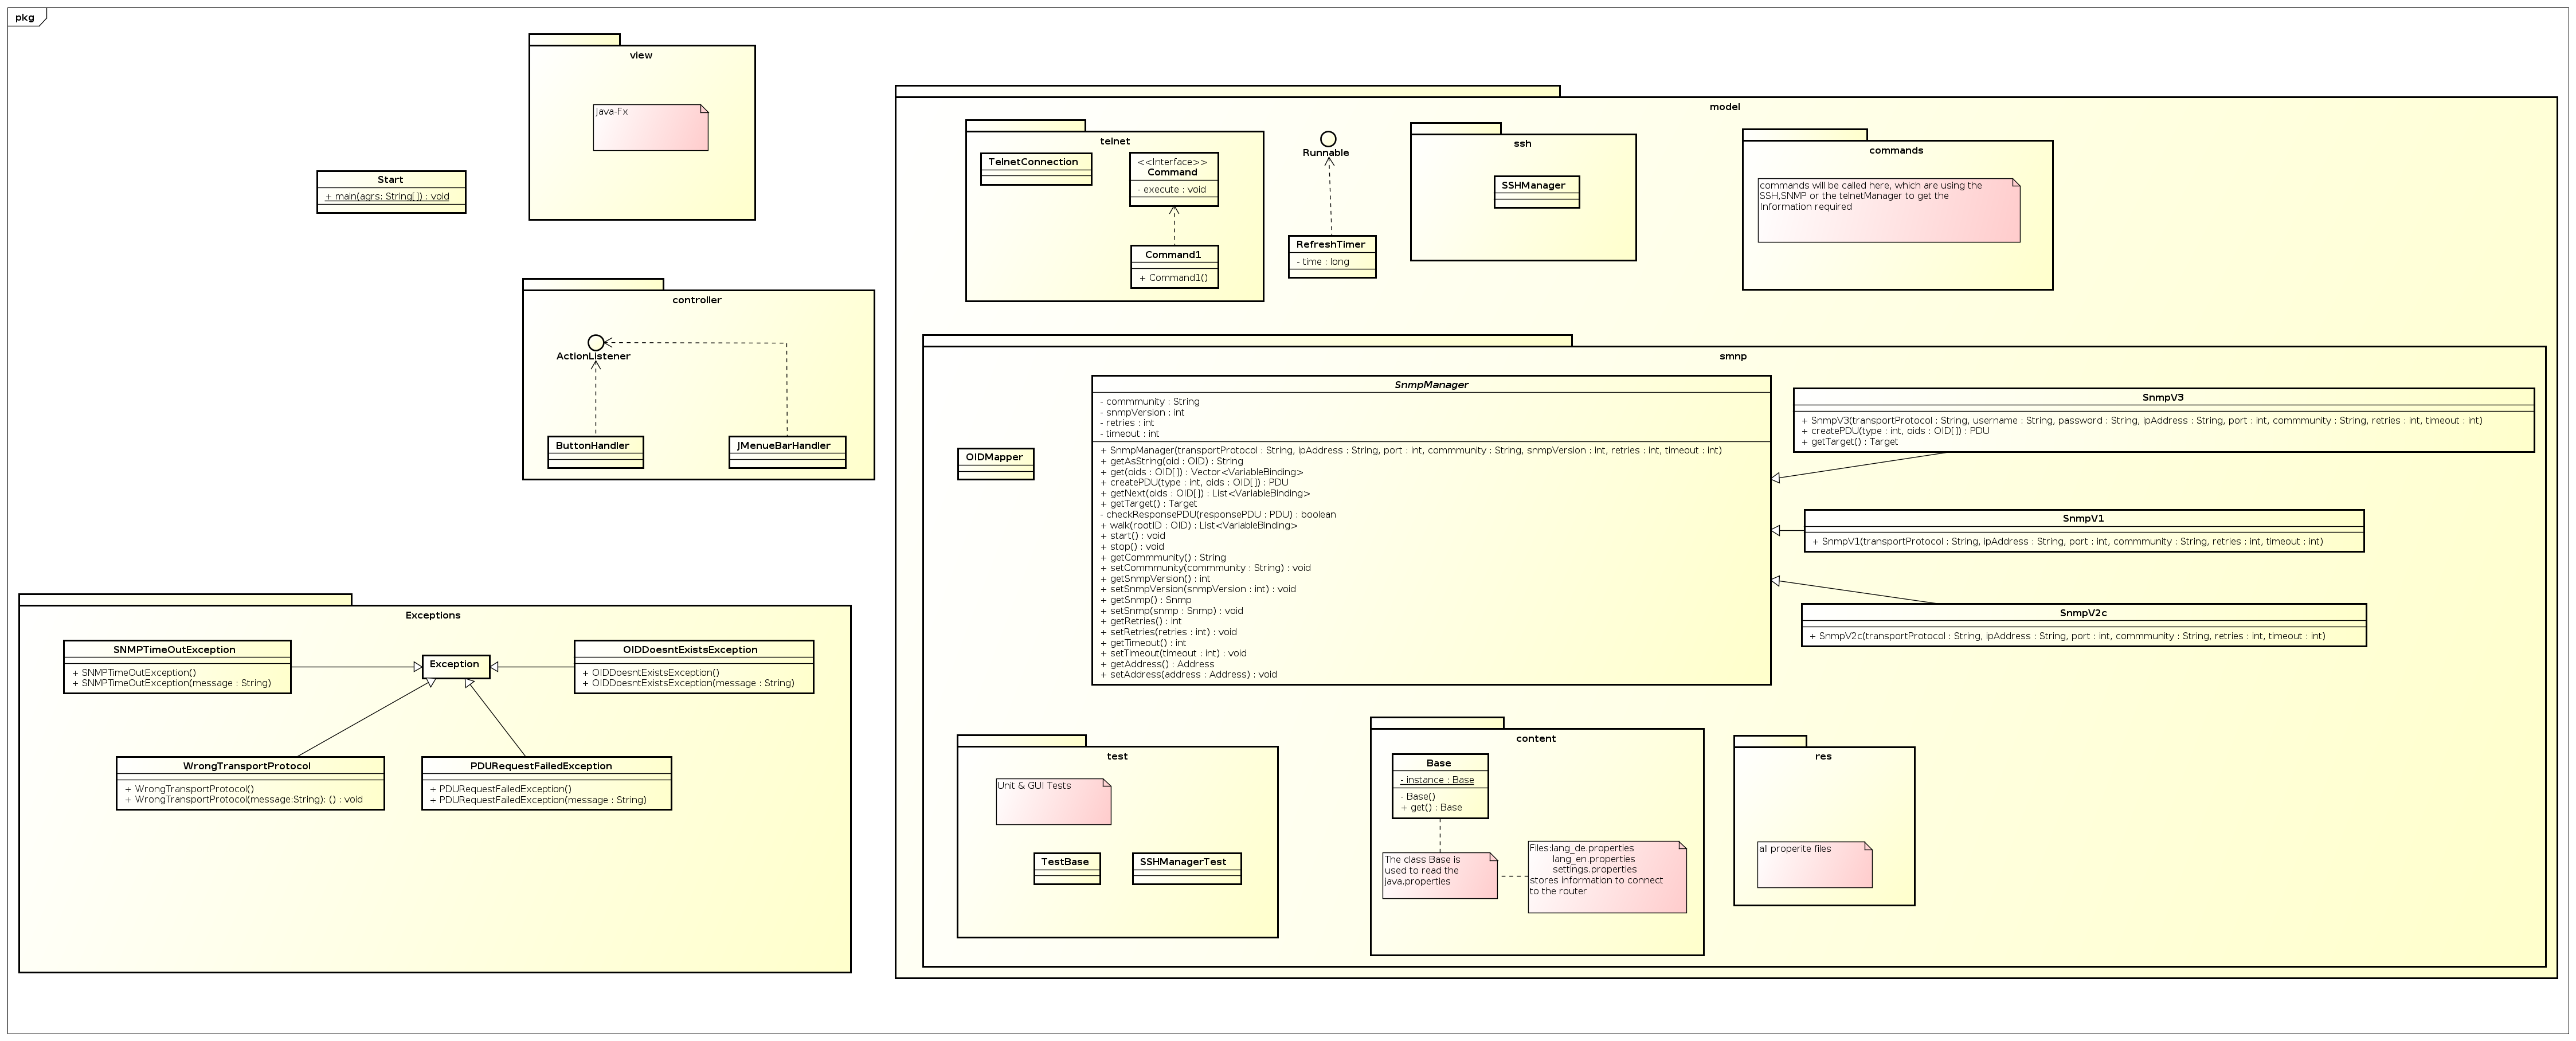
\includegraphics[width=1.0\textwidth]{RTNUmlImage}
\end{figure}

\chapter{Results and Defeats}
%There have been a whole lot of defeats but also a whole lot of results. The most Defeats where either Problems caused by Threads (a second Thread wehre just the first one should've been resumed, mixing up the variables for stopping the Thread and just let him do nothing for some Time and also some Thread suspends for a fixed time that weren't fully well matched) and the Server-Client communication. The communication Problems could often be fixed by updating either the Client or the Server to the newest version. \\
%The Design was completly done for TCP-communication only and we needed to implement some workarounds for UDP-support.\\
%The Basic features worke really quick how they where supposed to be but it needed quite some work for meeting some of the specifikations and to get everything Work together, wich wouldn't have been if there where a better Design and a better communication about the Design in the first place. For example, the Connection Interface is missing some possibillities that would made some things much easier and also the coexistence of the User- and the BufferedConnection-Thread caused some Problems, especially in kombination with the Connection-Wrapping, wich weher solved eventually but with some extra work. \\
%But eventually everithing worked fine, it was a really good feeling after every new bit that started doing what it should do an we also now understand the logik behind Threads and Sockets better and the benefits of a well done and well thought class Diagramm.

\chapter{Testreview}
\subsection{Main Unittest list}
coming soon\\

\subsection{Systemtest}


\chapter{Sources}
http://sourceforge.net/p/devmon/mailman/message/20347524/\\
http://www.oidview.com/mibs/3224/NETSCREEN-POLICY-MIB.html\\
http://www.circitor.fr/Mibs/Html/NETSCREEN-POLICY-MIB.php\\
\end{document}